\section{Segmentação}


Com um volume de dados grande disponível, uma possibilidade para as empresas é conseguir reconhecer certos padrões. Por exemplo, conhecendo o perfil dos clientes, é possível adotar estratégias adequadas para cada segmento, principalmente quando o público alvo é composto por clientes muito heterogêneos. Segundo \citeonline[p. 257]{KOTLER}, ``segmentação de mercado é o ato de dividir um mercado em grupos distintos de compradores com diferentes necessidades e respostas''.

\begin{citacao} 
Um bom agrupamento exibe a característica de que objetos associados ao mesmo grupo são bastante similares, ao mesmo tempo em que objetos associados a grupos diferentes exibem uma baixa similaridade. Aplicações diretas da análise de grupos incluem segmentação de clientes ou de produtos, agrupamento de genes em um experimento de micro-array, organização dos resultados de uma consulta enviada a um mecanismo de busca da WEB, etc.
\cite{BEZERRA} \end{citacao}

Com a segmentação e os grupos definidos, é possível realizar uma análise descritiva para traçar um padrão no comportamento dos dados. 

% ---
\subsection{K Médias}
% ---

O K Médias é um algoritmo de \emph{machine learning} não supervisionado relativamente simples, podendo ser utilizado para resolver problemas de clusterização. Para \citeonline{MacQueen}, trata-se de um método que tem para uma quantidade k de \emph{clusters} pré definida, o objetivo de definir k centróides\footnotemark \footnotetext{centróide é um conceito muito utilizado em geometria e física e representa um ponto médio ou um centro de massa de uma representação. No caso de K Médias, considerando que as informações são transformadas em vetores, seria um ponto médio da informação}, um para cada \emph{cluster}, tal que o conjunto de dados possa ser repartido de forma eficiente. Para um conjunto de observações \begin{math}(x_{1}, x_{2}, ..., x_{n})\end{math}, onde 

\begin{equation}
\label{eq:media}
\underset{S}{\arg\max} \sum_{i=1}^{k} \sum_{x \in S_{i}}\left \| x - \mu_{i} \right \|^{2}
\end{equation}

onde \begin{math}\mu_{i}\end{math} é a média dos pontos em \begin{math}S_{i}\end{math}

O algoritmo minimiza a função objetiva usando o princípio dos mínimos quadrados. Por conta disso, é sensível a \emph{ouliers} e ruídos. O pseudo algoritmo do K Médias seria estes passos:\\

\begin{algorithm}[H]
\SetAlgoLined
 1. Defina uma inicialização inicial aleatória usando k \emph{clusters}\;
 \While{Não houve convergência}{
   2. Atribua para cada ponto do conjunto de dados um \emph{cluster} mais próximo\;
   3. Redefina a posição do centróide de cada \emph{cluster} como um ponto médio de todos os pontos do \emph{cluster}\;
 }
 \caption{K Médias}
\end{algorithm}

\vspace{5mm}


\begin{figure}[!ht]
\caption{Evolução da execução do algoritmo de K Médias }
\centerline{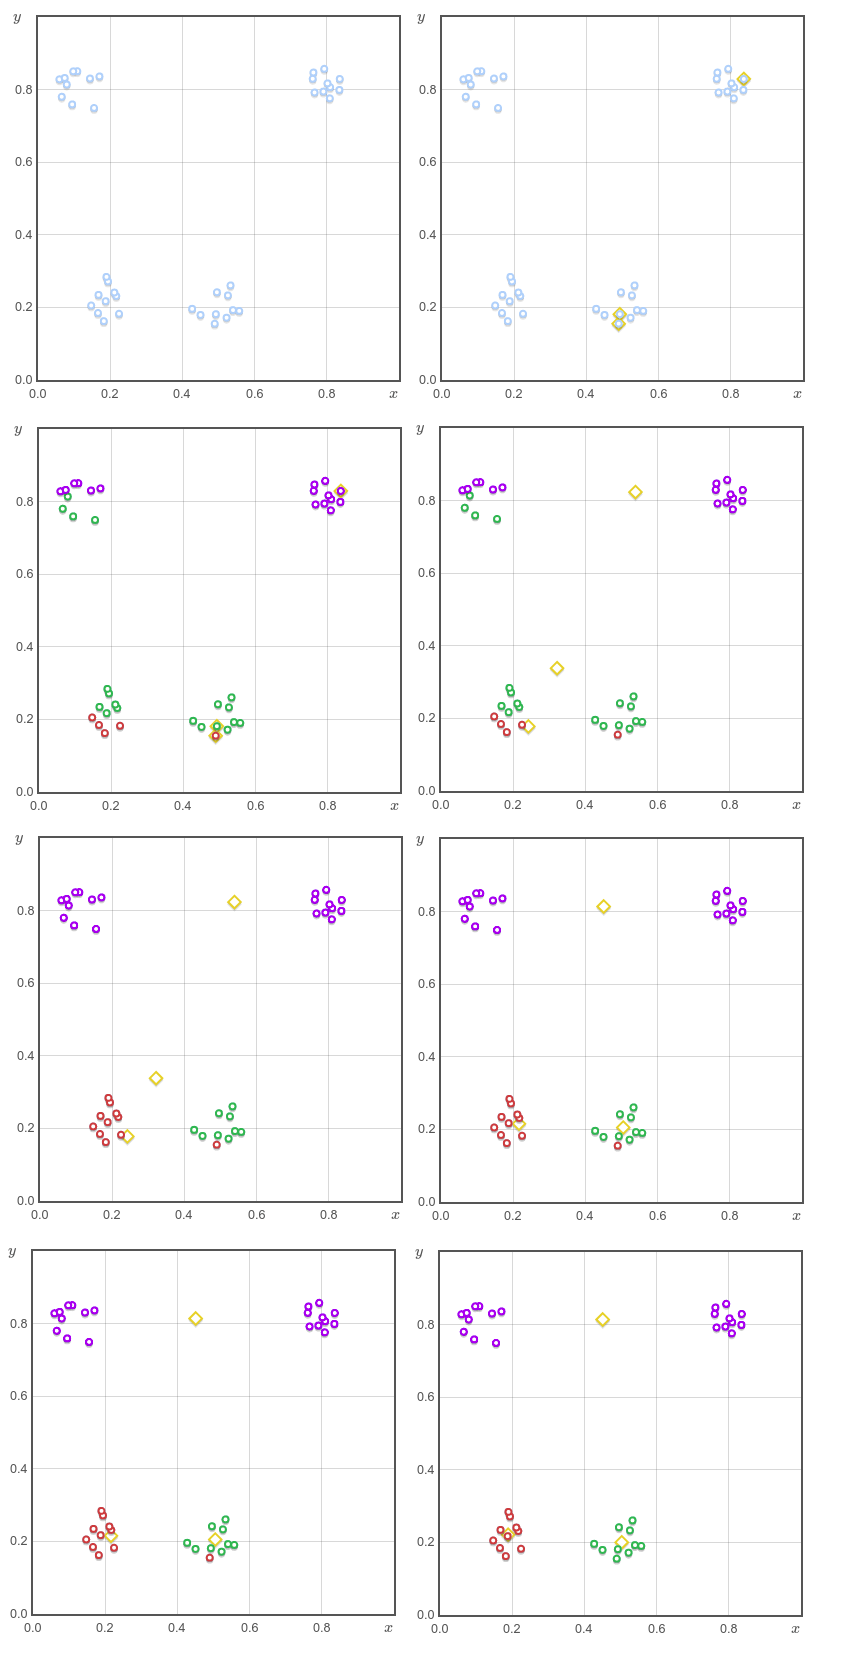
\includegraphics[width=0.5\textwidth]{img/k-means}}
\fonte{Extraído de \cite{kmeans-step}}
\end{figure}



A localização desses centróides deve ser o mais afastado entre si possível. A partir de uma posição inicial dos centróides, o próximo passo é, então, associar todos pontos do conjunto de dados com o centróide mais próximo. Com os pontos associados, recalcula-se k novos centróides como baricentros dos \emph{clusters} anteriores, repetindo esses passos até que os novos centróides sejam gerados muito próximos do passo anterior. 



